\section{Google Maps API}

Google Maps allows us to display maps on their website. The Google Maps Application Programming Interface (Google Maps API) is a set of tools and methods used to include Google Maps' features in an application, and overlay our own data over them; the Google Maps API allows to customize maps and the information displayed on these maps.

The Google Maps API is composed of a wide array of specialized APIs :

\begin{itemize}
	\item JavaScript API v3 : Embed an interactive map in a web page using Javascript;
	\item Maps for Work : Additionnal features to the standard Google Maps API devoted to business requirements and support;
 	\item Google Maps SDK for iOS : Add an interactive map to an iOS application;
  \item Google Maps Android API : Add an interactive map to an Android application;
	\item Google Maps API Web Services : HTTP interfaces to Google services, allowing user to invoke Google Maps data through URL requests; this feature consists of a large set of other APIs, like the ones following;
	\item Google Maps Embed API : Embed an interactive map or street view panorama in a web page with HTTP requests;
 	\item Google Places API : Display information about geographic locations, or points of interest; it can be used to give users contextual real-time information about their geographical position, and search for information about local businesses and monuments;
 	\item Google Maps Image APIs : Set of APIs to embed a Google Maps static image or Street View imagery in a web page without JavaScript.
\end{itemize}

As we can see, the Google Maps API is rather complete and gives access to a large range of features, with specifical APIs for each of this features. As part of our project, we will focus on the retrieving of informations about locations using the Place API, creating an interactive map using the Maps Android API, and including functionnalities and customized data to our application with Google API Web Services.

\subsection{Google Maps Android API}
\paragraph{Add a Map to the application}The Google Maps API allows us to simply implement a map in our application through an XML layout file, and activity Java file. It provides several objects to organize the initial layout. At its initial state, our map does not contain any personalized content, tiles are empty, and icons are not yet clickable.
The map object in the application is modeled by the \textit{GoogleMap} class. This class handles the following operations : 
\begin{itemize}
	\item Connection to the Google Maps online services;
	\item Downloading map tiles;
	\item Displaying tiles on the screen;
	\item Displaying controls;
	\item Zoom.
\end{itemize}
It is possible to add our own behaviour in addition to the previous automatic operations, by providing new methods to the \textit{GoogleMap} object.Within the UI, a map will be represented by either a \textit{MapFragment} or \textit{MapView} object.

The initial state of the map is entirely configurable : we can change the camera position, the map type, the available controls and gestures; this configuration is done using an XML layout file, or programmatically if the insertion of the map was done through the activity Java file.

\paragraph{Drawing on the Map} This section provide all the tools we need to add customizable markers to our map. Markers have several properties that allow us to personnalize their behaviour (draggable, icon, anchor, visible...). Listeners to marker-related events are provided by the API. Info windows can be anchored to a marker to display information on a location. Info Windows are customizable, and can be assiocated to an event if clicked.
\begin{figure}[h!]
	\centering
	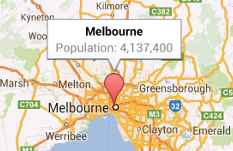
\includegraphics[scale=0.8]{input/marker-infowindows.png}
	\caption{Google Maps marker and Info Window}
	\label{fig:marker}
\end{figure}
\newpage
The Google Maps API also offers to add shapes to the map, using \textit{Polyline}, \textit{Polygon} and \textit{Circle} objects. As always, properties associated to these objects allow us to customize them. Finally, Ground and Tile overlays are images fixed to the map, allowing even more customization.

\paragraph{Interaction with the Map} The API provides UI controls that allows users to interact with the map. There are built-in zoom controls, a compass, the "My location" button which focus the map on the current user's location (if localization is enabled), and a toolbar which displays icons that provide access to a map view or directions. Map gestures are enabled by default, like tilt, zoom, rotate and scroll. Events associated to gesture are programmable.

\paragraph{Location Services} Thanks the GPS of the mobile device, and localization through mobile and wireless network, mobiles devices provide a set of localization technologies usable by our application. The Google Maps Android API provides the programming tools needed to benefit from those features. To add location awareness to our application, we must use the Google Play services Location API. This API lets us determine the location of the device, listen to locatoin changes, and monitor geofences.

\subsection{Google Maps API Web Services} The Google Maps API Web Services provides a large set of Web-oriented APIs using HTTP interfaces to Google services to provide geographic data to our application. We will only overview the APIs that seems the most relevant to the application we want to develop. All those APIs come with a large number of optional parameters to make them fit to our goal of use.
\paragraph{Directions API} This service calculates directions between different locations, for static adresses. Dynamic direction calculation are provided in the JavaScript API.

\paragraph{Distance Matrix API} This services provides travel distance and time between the elements of a matrix of origins and destinations.

\paragraph{Geocoding API} The Geocoding API provides tools to convert addresses into geographical coordinates and vice versa.

\subsection{Google Places API}The Google Place API provides a \textit{PlacePicker} UI widget that allows our application's users to select a place on the map. It also helps to get the last known current location and return a list of likely places for this location, and their likelihood. More importantly, this API retrieve and display informations about a place using the Google Play services.